\documentclass[10pt,oneside]{article}

\usepackage[T1]{fontenc}

\usepackage[paper=a4paper,margin=2cm,bottom=2.5cm]{geometry}
\usepackage[sfdefault,light,condensed]{roboto}
\usepackage[export]{adjustbox}
\usepackage[usenames,dvipsnames,table]{xcolor}

\usepackage{amsmath,amssymb,array,fancyhdr,graphicx,enumitem,lastpage,listings,lstautogobble,multicol,tabularx,textcomp,titlesec}
\usepackage{mathtools}

\setlength\parindent{0cm}
\renewcommand\headrule{}
\setlength{\footskip}{1.25cm}


\pagestyle{fancy}

\usepackage{fontawesome,subcaption,tikzsymbols}

% Add some padding to all table cells.
\setlength\extrarowheight{1pt}

%\newcommand{\boxwidth}{\dimexpr\linewidth - 2pt}
\newcommand{\boxwidth}{\linewidth}

\definecolor{BoxHeaderBG}{RGB}{50, 50, 50}
\definecolor{BoxHeaderText}{RGB}{220, 220, 220}

\definecolor{QuestionHeaderBG}{RGB}{200, 200, 200}
\definecolor{QuestionHeaderText}{RGB}{0, 0, 0}

\newcommand{\BoxHeader}[2]{
    \multicolumn{#1}{| >{\bfseries\footnotesize\cellcolor{BoxHeaderBG}\arraybackslash}l |}{
        \textcolor{BoxHeaderText}{#2}
    }
}

\newcounter{QuestionCounter}

\newcommand{\Question}[2]{
    \stepcounter{QuestionCounter}
    \begin{tabularx}{\boxwidth}{|X|}
        \hline
        \cellcolor{QuestionHeaderBG}{\footnotesize\bfseries \textcolor{QuestionHeaderText}{Question \#\theQuestionCounter}} {\em \textcolor{QuestionHeaderText}{#1}} \\\hline
        \ \\[#2]\hline
    \end{tabularx}

    \medskip
}

\newcommand{\FeelQuestion}{
    \stepcounter{QuestionCounter}
    \newcolumntype{F}{>{\centering\arraybackslash}X}
    \begin{tabularx}{\boxwidth}{| F F F |}
        \hline
        \multicolumn{3}{| >{\hsize=\dimexpr3\hsize+4\tabcolsep+2\arrayrulewidth\relax}X |}{
            \cellcolor{QuestionHeaderBG}{\footnotesize\bfseries \textcolor{QuestionHeaderText}{Question \#\theQuestionCounter}} {\em \textcolor{QuestionHeaderText}{Select the option which best reflects how confident you are in applying what you have learend in this lesson.}}}\\\hline
        & & \\[-8pt]
        \Sadey[5][orange] & \Neutrey[5][gray] & \Smiley[5][cyan] \\\hline
    \end{tabularx}

    \medskip
}

\lhead{\tiny\texttt{U\UnitNumber: \UnitTitle\\L\LessonNumber: \LessonTitle}}
\rhead{\tiny\texttt{[DPCS/\CourseLevel/U\UnitNumber/\LessonNumber]\\ }}

\lfoot{
\includegraphics[height=2cm,valign=c]{Files/logo}}
\cfoot{\footnotesize \LessonTitle/DPCS/\CourseLevel/U\UnitNumber/L\LessonNumber/\thepage/\pageref{LastPage}\\Woodstock School/Mussoorie, Uttarakhand, India}
\rfoot{
\includegraphics[height=2cm,valign=c]{Files/ib-world-school-logo-1-colour}}


\def\CourseLevel{LL}

\def\UnitNumber{01}
\def\UnitTitle{The Computer}

\def\LessonNumber{04}
\def\LessonTitle{The Operating System}

\begin{document}
    %Lesson Title
    \begin{center}
        \Large\bfseries \LessonTitle
    \end{center}

    % Objectives List
    \begin{tabularx}{\boxwidth}{|>{\small\raggedleft\bfseries\arraybackslash}p{0.1\textwidth} >{\small\arraybackslash}X |}
        \hline
        \BoxHeader{2}{Objective} \\\hline
        2.1.6 & Describe the main functions of an operating system. \\\hline
    \end{tabularx}

    % Opening Exercise
    \section*{Before You Begin}


    \vfill

    \pagebreak
    
    % Definitions
    \section*{Important Terms}
    \begin{tabularx}{\boxwidth}{| >{\bfseries\arraybackslash}p{0.3\textwidth} | X | }
        \hline
        \BoxHeader{1}{Term} & \BoxHeader{1}{Definition} \\\hline
        Device Driver & \\[2cm]\hline
        Hardware Abstraction Layer & \\[2cm]\hline
        Kernel & \\[2cm]\hline
        Kernel Space & \\[2cm]\hline
        Operating System (OS) & \\[2cm]\hline
        User Space & \\[2cm]\hline
    \end{tabularx}

    \pagebreak

    % Technical Background
    \section*{Technical Background}

    \subsection*{The Role of the Operating System}
    The following diagram is an abstraction showing where the operating system exists in relation to the user applications and the system hardware.

    \medskip
    \begin{figure}[h]
        \centering
        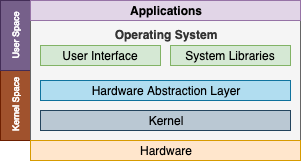
\includegraphics[width=8cm]{Extras/operating_system_simple}
        \caption{A simple view of the software layers of a computer system.}
    \end{figure}

    \subsubsection*{Notes}

    \vfill

    \Question{What benefit does the segregation of memory space for core kernel operations from user-initiated operations have on the stability of a computer system? Are there any drawbacks to this model?}{4cm}

    \pagebreak

    \subsection*{Monolithic vs. Microkernel Operating Systems}

    The following two diagrams show a sample of fundamental services offered by the operating system, and where they would exist within a monolithic or microkernel operating system architecture.

    \medskip
    \begin{figure}[h]
        \centering
        \begin{subfigure}{0.45\boxwidth}
            \centering
            \caption*{\bfseries Monolithic}
            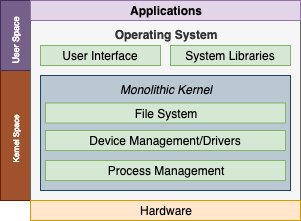
\includegraphics[width=6cm]{Extras/operating_system_monolithic}
        \end{subfigure}
        \begin{subfigure}{0.45\boxwidth}
            \centering
            \caption*{\bfseries Microkernel}
            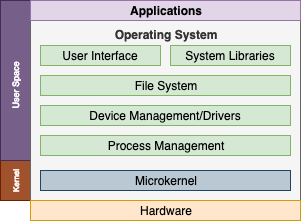
\includegraphics[width=6cm]{Extras/operating_system_microkernel}
        \end{subfigure}
    \end{figure}
    
    \subsubsection*{Notes}

    \vfill

    \Question{Monolithic kernels run a higher risk of instability due to all services being included in a single process. Despite this, operating systems which are considered \emph{more stable} and \emph{more secure}, such as Linux, generally use monolithic kernels, while systems considered \emph{less stable} and \emph{less secure}, such as Mac OSX and Windows, use microkernels. Why do you think this contradiction exists?}{4cm}

    \pagebreak
    % Developing Technical Skills
    \section*{Developing Technical Skills}
    \subsubsection*{Activity Title}

    \vfill

    \Question{Third Question}{4cm}

    \pagebreak

    % Reflections
    \section*{Reflections}

    \Question{Significant advances and changes in computer hardware frequently require updates to an operating system's kernel, particularly in monolithic systems such as Linux. Do you think operating system vendors should push for more standardization of computer hardware? Why or why not?}{4cm}

    \Question{Windows Vista and newer require kernel-mode device drivers to be ``digitally signed'' by Microsoft. This process verifies a drivers use and authenticity. Why do you think Microsoft implemented this security measure?}{4cm}

    \Question{Describe at least one new thing you have learned from this lesson. How might you apply this knowledge in the future?}{3.5cm}

    \FeelQuestion

    \Question{What further questions do you still have about this lesson's content?}{3.5cm}
\end{document}